%
% section 6.1.1
%
\subsection{Χώρος Ονομάτων του DNS}

Το Διαδίκτυο χωρίζεται σε εκατοντάδες διαφορετικές περιοχές που ονομάζονται \emph{domains}. Οι περιοχές χωρίζονται σε υποπεριοχές (subdomains) και αυτές σε άλλες κ.ο.κ. κάθε μια με ένα ή περισσότερους υπολογιστές (hosts).

Οι περιοχές μπορούν να αναπαρασταθούν με ένα δέντρο. Τα ονόματα σχηματίζουν μια ιεραρχία με τρόπο που είναι μοναδικά και μπορούν να απομνημονευθούν σχετικά εύκολα. Για κάθε περιοχή ορίζεται κάποιος αρμόδιος ο οποίος διαχειρίζεται τον αντίστοιχο εξυπηρετητή DNS και μπορεί να προσθέσει ή να επεξεργαστεί υποπεριοχές (subdomains) και υπολογιστές (hosts). Κάθε κόμβος στο σύστημα DNS αναπαριστά ένα όνομα DNS (DNS Name). Κάθε κλαδί κάτω από ένα κόμβο είναι μια περιοχή DNS (DNS Domain) και μπορεί να περιέχει υποπεριοχές και υπολογιστές.   

\begin{figure}[!ht]
  \centering
  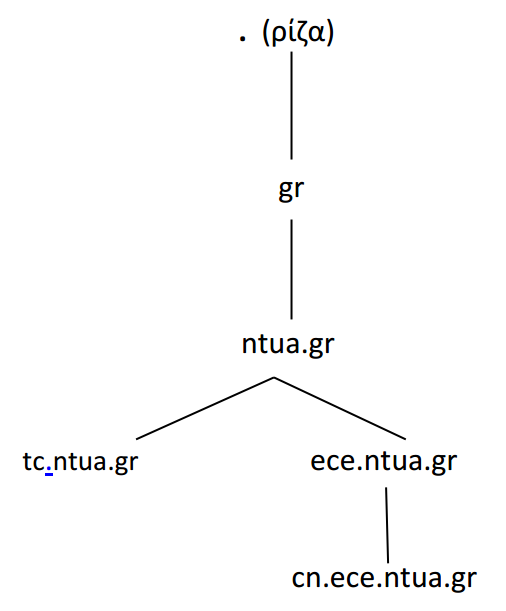
\includegraphics[width=0.75\textwidth]{images/chapter6/6-0}
  \caption {\textsl{Παράδειγμα Περιοχών DNS}}
  \label{6-0}
\end{figure}

Στην κορυφή της ιεραρχίας του DNS είναι η ρίζα που συμβολίζεται με μια τελεία ``.'' (σχήμα \ref{6-0}). Επίσημος διαχειριστής της ρίζας είναι η \emph{IANA, Internet Assigned Numbers Authority}. Κάτω από τη ρίζα υπάρχουν οι περιοχές \emph{ανώτατου επιπέδου} (top level domains, ή περιοχές βασικού επιπέδου ή βασικές περιοχές). Αρχικά (το 1988) υπήρχαν οι περιοχές που φαίνονται στο σχήμα \ref{6-1}.

\begin{figure}[!ht]
  \centering
  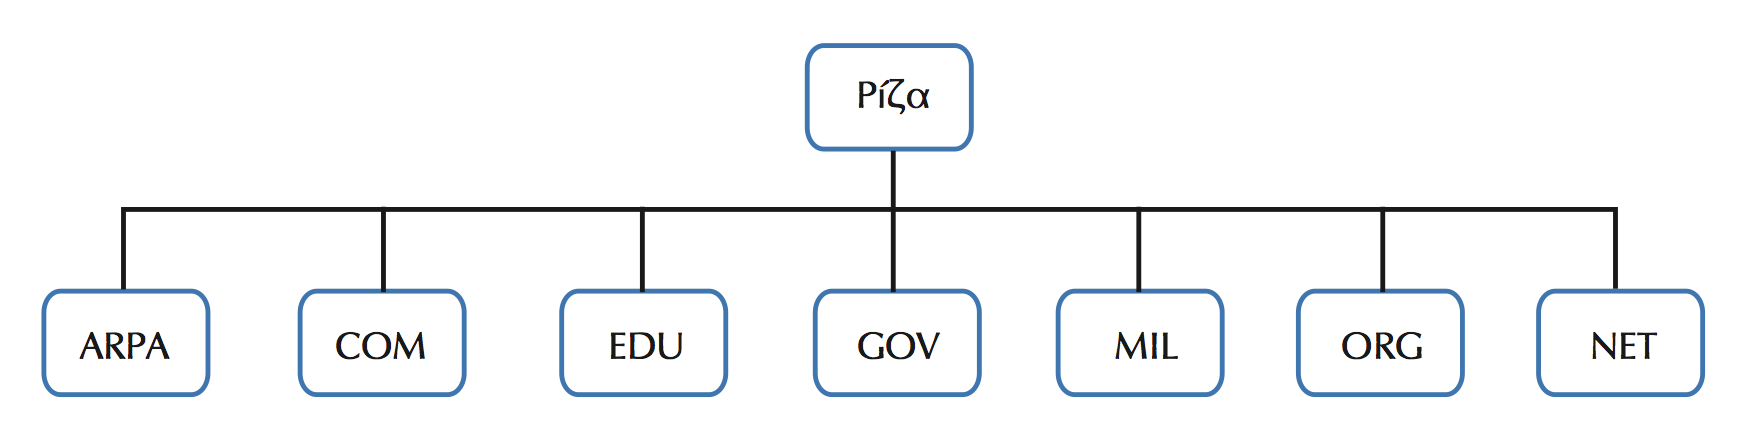
\includegraphics[width=0.95\textwidth]{images/chapter6/6-1}
  \caption {\textsl{Περιοχές DNS 1ου Επιπέδου}}
  \label{6-1}
\end{figure}

Οι καταλήξεις στο πρώτο επίπεδο δηλώνουν:

\begin{itemize}
\item \textbf{.arpa}: Ειδικοί οργανισμοί διαδικτύου
\item \textbf{.com}: Εταιρίες (εμπορικές)
\item \textbf{.edu}: Εκπαιδευτικά ιδρύματα, πανεπιστήμια κλπ
\item \textbf{.gov}: Κυβερνητικοί οργανισμοί και υπηρεσίες
\item \textbf{.mil}: Στρατιωτικοί οργανισμοί
\item \textbf{.net}: Κέντρα διαχείρισης δικτύου
\item \textbf{.org}: Μη κερδοσκοπικοί οργανισμοί και γενικά οτιδήποτε δεν μπορεί να κατηγοριοποιηθεί σε μια από τις παραπάνω κατηγορίες.
\end{itemize}

Αργότερα προστέθηκαν περιοχές για κάθε χώρα (π.χ. .gr, .uk, .fr κλπ) και κάποιες επιπλέον περιοχές (όπως .biz, .post, .info κλπ.). Η διαχείριση τους (εκτός από την .int και .arpa) έχει εκχωρηθεί από την IANA σε άλλους οργανισμούς.

Κάτω από κάθε περιοχή πρώτου επιπέδου υπάρχει δεύτερο επίπεδο που προσδιορίζει την εταιρία ή τον οργανισμό στον οποίο ανήκει το δίκτυο. Οι περιοχές αυτές ονομάζονται \emph{2ου επιπέδου} και κάθε μια είναι μοναδική. 

Όταν μια εταιρεία ή οργανισμός κατοχυρώνει ένα domain, αναλαμβάνει και τη διαχείριση του αντίστοιχου χώρου ονομάτων. Μπορεί να αναθέσει σε μια εταιρία παροχής υπηρεσίών Internet να συντηρεί την περιοχή ή μπορεί να διαθέτει δικούς της εξυπηρετητές DNS. Σε κάθε περίπτωση ο κάτοχος του χώρου θα πρέπει να διαθέτει τον εξοπλισμό ώστε να απαντά σε ερωτήματα σχετικά με τους υπολογιστές που ανήκουν στη περιοχή του καθώς και σε όποιες υποπεριοχές δημιουργήσει ο ίδιος.

\begin{figure}[!ht]
  \centering
  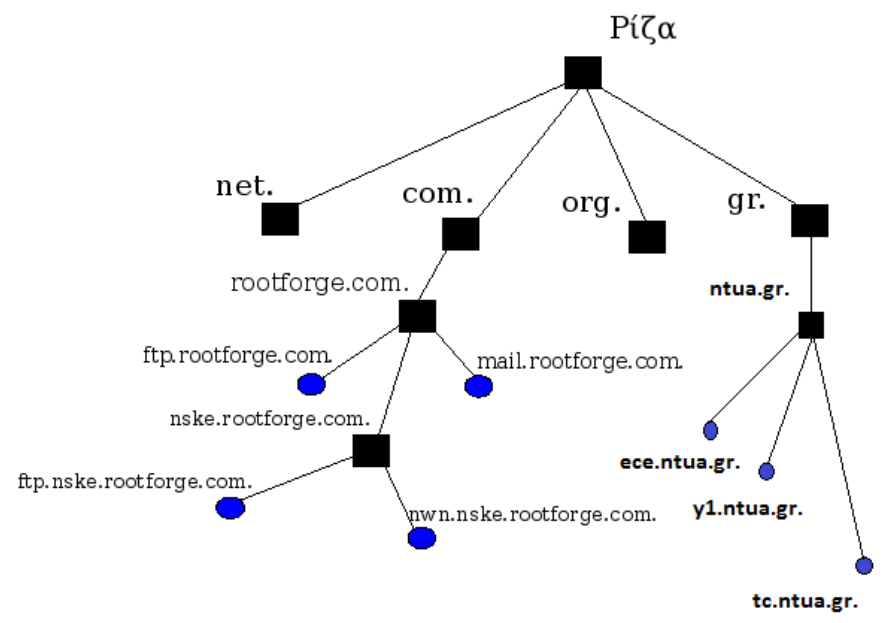
\includegraphics[width=0.95\textwidth]{images/chapter6/6-2}
  \caption {\textsl{Ιεραρχική Οργάνωση Χώρου DNS}}
  \label{6-2}
\end{figure}

Στο σχήμα \ref{6-2} φαίνεται μια τέτοια οργάνωση. Στην κορυφή του δέντρου βρίσκεται η ρίζα που τη διαχειρίζεται η ΙΑΝΑ. Μια από τις βασικές περιοχές (1ου επιπέδου) είναι και η \textbf{.gr} για την οποία είναι υπεύθυνο το \href{https://grweb.ics.forth.gr/public/}{ΙΤΕ, Ίδρυμα Τεχνολογίας και Έρευνας}. Στο δεύτερο επίπεδο συναντάμε την περιοχή \emph{ntua.gr} η οποία ανήκει στο Εθνικό Μετσόβιο Πολυτεχνείο (ΕΜΠ). Το όνομα y1.ntua.gr προσδιορίζει τον υπολογιστή y1 στο δίκτυο του ΕΜΠ.

Σε γενικές γραμμές, όταν βλέπουμε ένα πλήρες όνομα DNS, το πλέον αριστερό τμήμα προσδιορίζει τον υπολογιστή και το πλέον δεξιό την περιοχή βασικού επιπέδου. Για παράδειγμα, το παρακάτω είναι έγκυρο όνομα:

\begin{center}
ektor.tc.ntua.gr
\end{center}

όπου:

\begin{itemize}
\item[-]ektor: Είναι το όνομα του υπολογιστή
\item[-].tc: Είναι το όνομα της περιοχής 3ου επιπέδου
\item[-].ntua: Είναι το όνομα της περιοχής 2ου επιπέδου
\item[-].gr: Είναι το όνομα της περιοχής 1ου (βασικού) επιπέδου
\end{itemize}

Σημειώνουμε εδώ ότι μπορεί να υπάρχουν επίπεδα και πάνω από το 3ο, αλλά δεν τα συναντάμε συχνά, τουλάχιστον όχι σε εξυπηρετητές ιστοσελίδων. Δεν είναι όμως σπάνιο για μια επιχείρηση να έχει δομήσει το εσωτερικό της δίκτυο σε περισσότερα από τρία επίπεδα.

Ένα πιο συνηθισμένο παράδειγμα DNS για ένα υπολογιστή που εκτελεί χρέη εξυπηρετητή ιστοσελίδων είναι το παρακάτω:

Όταν συνδεθήκατε για να κατεβάσετε αυτό το βιβλίο, χρησιμοποιήσατε τη διεύθυνση:

\begin{center}
www.freebsdworld.gr
\end{center}

\begin{itemize}
\item Για να συνδεθείτε, ο αναλυτής (resolver) στον υπολογιστή σας πρέπει να μάθει τη διεύθυνση IP της παραπάνω τοποθεσίας. Το ερώτημα τίθεται στον εξυπηρετητή DNS του παροχέα Internet που χρησιμοποιείτε.
\item Ο DNS του παροχέα σας ρωτάει αρχικά τον εξυπηρετητή που είναι υπεύθυνος για την περιοχή ``.gr''. Ο εξυπηρετητής αυτός γνωρίζει μόνο ποιος  εξυπηρετητής DNS είναι υπεύθυνος για την περιοχή 2ου επιπέδου ``freebsdworld.gr'' και τον παραπέμπει προς αυτόν.
\item Ο εξυπηρετητής του παροχέα επικοινωνεί με τον εξυπηρετητή DNS που είναι υπεύθυνος για την περιοχή ``freebsdworld.gr'' για να μάθει τη διεύθυνση IP του μηχανήματος με όνομα ``www''. Την απάντηση αυτή στέλνει στο δικό σας ερώτημα (και ταυτόχρονα την αποθηκεύει για μελλοντική χρήση).
\end{itemize}

Στην παραπάνω διεύθυνση, το ``www'' αποτελεί το όνομα του υπολογιστή που εκτελεί την υπηρεσία ιστοσελίδων (web server). Όπως φαίνεται και από το παράδειγμα μας, η βάση DNS είναι κατανεμημένη και διαφορετικοί υπολογιστές είναι υπεύθυνοι για τις αντίστοιχες περιοχές. Οι εξυπηρετητές DNS βρίσκονται σε διαφορετικά σημεία και συνεργάζονται μεταξύ τους για να απαντήσουν στα ερωτήματα.